% ============================================================
%  Cliff Walking -- LaTeX Beamer Presentation
%  Compile:  pdflatex cliff_walking_slides.tex  (run twice)
% ============================================================
\documentclass[aspectratio=169,8pt]{beamer}
\usepackage[utf8]{inputenc}
\usepackage[T1]{fontenc}

% Theme
\usetheme{Madrid}
\usecolortheme{seahorse}
\usefonttheme{professionalfonts}
\setbeamertemplate{navigation symbols}{}
\setbeamertemplate{footline}[frame number]

% Packages
\usepackage{amsmath,amssymb,amsthm}
\usepackage{mathtools}
\usepackage{bm}
\usepackage{listings}
\usepackage{xcolor}
\usepackage{tikz}
\usetikzlibrary{arrows.meta,positioning,calc}
\usepackage{booktabs}
\usepackage{array}
\usepackage{multirow}

% Colours
\definecolor{cliffRed}   {RGB}{192, 57, 43}
\definecolor{goalGreen}  {RGB}{ 39,174, 96}
\definecolor{startBlue}  {RGB}{ 41,128,185}
\definecolor{safeGray}   {RGB}{236,240,241}
\definecolor{codeBack}   {RGB}{248,249,250}
\definecolor{codeBorder} {RGB}{189,195,199}
\definecolor{keyBlue}    {RGB}{ 52, 73,110}
\definecolor{commentGray}{RGB}{127,140,141}
\definecolor{stringGreen}{RGB}{ 39,174, 96}
\definecolor{mathBlue}   {RGB}{ 41,128,185}

% Listings
\lstdefinestyle{pycode}{
  language=Python,
  basicstyle=\ttfamily\scriptsize,
  keywordstyle=\bfseries\color{keyBlue},
  commentstyle=\itshape\color{commentGray},
  stringstyle=\color{stringGreen},
  backgroundcolor=\color{codeBack},
  frame=single,
  rulecolor=\color{codeBorder},
  breaklines=true,
  numbers=left,
  numberstyle=\tiny\color{commentGray},
  numbersep=4pt,
  xleftmargin=10pt,
  showstringspaces=false,
  tabsize=4,
  escapeinside={(*@}{@*)},
}
\lstset{style=pycode}

% Math shortcuts
\newcommand{\St}{\mathcal{S}}
\newcommand{\Act}{\mathcal{A}}
\newcommand{\Vopt}{V^{*}}
\newcommand{\piopt}{\pi^{*}}
\newcommand{\E}{\mathbb{E}}

% Title
\title[Cliff Walking RL]{\textbf{Cliff Walking}\\
  \large Mathematical Walkthrough of the PyCharm Project}
\subtitle{environment.py \quad value\_iteration.py \quad simulation.py}
\author{Reinforcement Learning}
\date{\today}

% ============================================================
\begin{document}
% ============================================================

\begin{frame}
  \titlepage
\end{frame}

\begin{frame}{Outline}
  \tableofcontents
\end{frame}

% ============================================================
\section{MDP Foundations}
% ============================================================

\begin{frame}{Markov Decision Process}
  A finite MDP is the tuple
  $\langle \St,\,\Act,\,\mathcal{T},\,\mathcal{R},\,\gamma \rangle$

  \begin{columns}[T]
    \column{0.52\textwidth}
    \begin{block}{Components}
      \begin{itemize}
        \item $\St = \{s_0,\ldots,s_{|\St|-1}\}$ \quad finite states
        \item $\Act = \{a_0,\ldots,a_{|\Act|-1}\}$ \quad finite actions
        \item $\mathcal{T}(s,a,s')=\Pr[S_{t+1}{=}s'\mid S_t{=}s,A_t{=}a]$
        \item $\mathcal{R}(s,a)$ \quad expected reward
        \item $\gamma\in[0,1)$ \quad discount factor
      \end{itemize}
    \end{block}
    \begin{block}{Objective}
      Find $\pi:\St\!\to\!\Act$ maximising the discounted return:
      \[
        G_t = \sum_{k=0}^{\infty}\gamma^{k}R_{t+k+1}
      \]
    \end{block}

    \column{0.44\textwidth}
    \begin{alertblock}{Markov property}
      \[
        \Pr[S_{t+1}\mid S_t,A_t,\ldots,S_0]
        = \Pr[S_{t+1}\mid S_t,A_t]
      \]
      The future depends \emph{only} on the current state
      and action -- not the full history.
    \end{alertblock}
    \begin{block}{Cliff Walking instance}
      \begin{tabular}{ll}
        $|\St|$ & $48$ cells \\
        $|\Act|$ & $4$ directions \\
        $\gamma$ & $0.99$ \\
      \end{tabular}
    \end{block}
  \end{columns}
\end{frame}

% ============================================================
\section{environment.py}
% ============================================================

\begin{frame}[shrink=5]{environment.py -- Grid and State Space}
  \begin{columns}[T]
    \column{0.50\textwidth}
    \begin{block}{State encoding}
      Grid: 4 rows $\times$ 12 columns $= 48$ cells.
      \[
        s \;=\; r\cdot 12 + c
        \;\in\; \{0,1,\ldots,47\}
      \]
      \[
        (r,c) \;=\; \bigl(\lfloor s/12\rfloor,\; s\bmod 12\bigr)
      \]
      \begin{itemize}
        \item $S_{\text{start}} = 3\cdot12+0 = 36$
        \item $S_{\text{goal}}  = 3\cdot12+11= 47$
        \item $\mathcal{C}=\{37,38,\ldots,46\}$ (cliff)
      \end{itemize}
    \end{block}
    \begin{block}{Action set $\Act$}
      \small
      \begin{tabular}{clc}
        \toprule
        Index & Name  & $(\Delta r,\Delta c)$ \\
        \midrule
        0 & Up    & $(-1,\;0)$ \\
        1 & Down  & $(+1,\;0)$ \\
        2 & Left  & $(0,-1)$   \\
        3 & Right & $(0,+1)$   \\
        \bottomrule
      \end{tabular}
    \end{block}

    \column{0.46\textwidth}
    \vspace{4pt}
    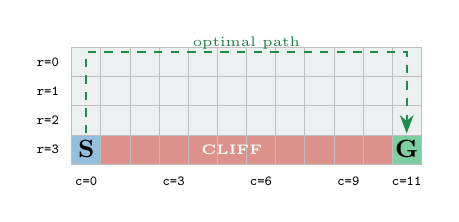
\begin{tikzpicture}[scale=0.37]
      \foreach \r in {0,1,2,3}{
        \foreach \c in {0,1,...,11}{
          \pgfmathsetmacro{\x}{\c}
          \pgfmathsetmacro{\y}{3-\r}
          \pgfmathparse{(\r==3)&&(\c>=1)&&(\c<=10)?1:0}
          \ifnum\pgfmathresult=1
            \fill[cliffRed!55] (\x,\y) rectangle (\x+1,\y+1);
          \else
            \pgfmathparse{(\r==3)&&(\c==0)?1:0}
            \ifnum\pgfmathresult=1
              \fill[startBlue!50] (\x,\y) rectangle (\x+1,\y+1);
            \else
              \pgfmathparse{(\r==3)&&(\c==11)?1:0}
              \ifnum\pgfmathresult=1
                \fill[goalGreen!60] (\x,\y) rectangle (\x+1,\y+1);
              \else
                \fill[safeGray] (\x,\y) rectangle (\x+1,\y+1);
              \fi
            \fi
          \fi
          \draw[gray!50, very thin] (\x,\y) rectangle (\x+1,\y+1);
        }
      }
      \node[font=\small\bfseries] at (0.5,0.5) {S};
      \node[font=\small\bfseries] at (11.5,0.5) {G};
      \node[font=\tiny\bfseries,white] at (5.5,0.5) {CLIFF};
      \draw[-{Stealth},thick,goalGreen!80!black,dashed]
        (0.5,1.05)--(0.5,3.85)--(11.5,3.85)--(11.5,1.05);
      \node[font=\tiny,goalGreen!70!black] at (6,4.15) {optimal path};
      \foreach \r in {0,1,2,3}
        \node[left,font=\tiny\ttfamily] at (-0.1,3.5-\r) {r=\r};
      \foreach \c in {0,3,6,9,11}
        \node[below,font=\tiny\ttfamily] at (\c+0.5,-0.1) {c=\c};
    \end{tikzpicture}

    \vspace{4pt}
    \begin{alertblock}{Wall-bounce rule}
      \[
        r' = \max(0,\min(3,\,r+\Delta r))
      \]
      Out-of-bounds moves keep the agent in place.
    \end{alertblock}
  \end{columns}
\end{frame}

% ----------------------------------------------------------
\begin{frame}[fragile,shrink=5]{environment.py -- State Encoding in Code}
  \begin{columns}[T]
    \column{0.50\textwidth}
    \begin{lstlisting}
NUM_ROWS, NUM_COLS = 4, 12
NUM_STATES  = 48  # |S|
NUM_ACTIONS = 4   # |A|

# s = 12*r + c
def rc_to_state(row, col):
    return row * NUM_COLS + col

# (r, c) = divmod(s, 12)
def state_to_rc(s):
    return divmod(s, NUM_COLS)

START_STATE  = 36  # (3, 0)
GOAL_STATE   = 47  # (3,11)
CLIFF_STATES = {3*12+c
                for c in range(1,11)}
    \end{lstlisting}

    \column{0.46\textwidth}
    \begin{block}{Why flat indexing?}
      The reward matrix and transition tensor
      are NumPy arrays:
      \[
        \mathcal{R}\in\mathbb{R}^{|\St|\times|\Act|}
        \quad
        \mathcal{T}\in\mathbb{R}^{|\St|\times|\Act|\times|\St|}
      \]
      Flat integer indices let us write
      \texttt{R[s,a]} and \texttt{T[s,a,s']}
      without any tuple conversion at runtime.
    \end{block}
    \begin{block}{Example indices}
      \small
      \begin{tabular}{lcc}
        \toprule
        Cell & $(r,c)$ & $s$ \\
        \midrule
        Start & $(3,0)$  & 36 \\
        Goal  & $(3,11)$ & 47 \\
        Cliff & $(3,1)$--$(3,10)$ & 37--46 \\
        \bottomrule
      \end{tabular}
    \end{block}
  \end{columns}
\end{frame}

% ----------------------------------------------------------
\begin{frame}[fragile]{environment.py -- Reward Function $\mathcal{R}(s,a)$}
  \begin{columns}[T]
    \column{0.48\textwidth}
    \begin{block}{Definition}
      Let $s'(s,a)$ be the wall-bounced next cell. Then:
      \[
        \mathcal{R}(s,a)=
        \begin{cases}
          -100 & s'(s,a)\in\mathcal{C}\\
          \phantom{-1}0  & s'(s,a)=S_G\\
          -1   & \text{otherwise}
        \end{cases}
      \]
    \end{block}
    \begin{block}{Shape: $\mathcal{R}\in\mathbb{R}^{48\times 4}$}
      \small
      \begin{tabular}{lcccc}
        \toprule
        State & $a{=}0$ & $a{=}1$ & $a{=}2$ & $a{=}3$ \\
        \midrule
        $s=36$ (Start) & $-1$ & $-100$ & $-1$ & $-100$ \\
        $s=24$ (safe)  & $-1$ & $-1$   & $-1$ & $-1$   \\
        $s=46$         & $-1$ & $-1$   & $-1$ & $0$    \\
        $s=47$ (Goal)  &  $0$ &  $0$   &  $0$ &  $0$   \\
        \bottomrule
      \end{tabular}
    \end{block}

    \column{0.48\textwidth}
    \begin{lstlisting}
# R shape: (48, 4)
R = np.full((48, 4), -1.0)

for s in range(48):
  row, col = state_to_rc(s)
  for a in range(4):
    dr, dc = ACTION_DELTAS[a]
    nr = max(0, min(3, row+dr))
    nc = max(0, min(11,col+dc))
    ns = rc_to_state(nr, nc)

    if ns in CLIFF_STATES:
      R[s, a] = -100.0
    elif ns == GOAL_STATE:
      R[s, a] = 0.0
    # else: stays -1.0
    \end{lstlisting}
    \begin{alertblock}{Note}
      The penalty is assigned to the \emph{action}
      that leads to the cliff, not to being in the
      cliff state -- consistent with standard
      tabular-MDP conventions.
    \end{alertblock}
  \end{columns}
\end{frame}

% ----------------------------------------------------------
\begin{frame}[fragile,shrink=5]{environment.py -- Transition Tensor $\mathcal{T}(s,a,s')$}
  \begin{columns}[T]
    \column{0.48\textwidth}
    \begin{block}{Deterministic dynamics}
      \[
        \mathcal{T}(s,a,s')=
        \begin{cases}
          1 & s'=f(s,a)\\
          0 & \text{otherwise}
        \end{cases}
      \]
      where the next-state function $f$ is:
      \[
        f(s,a)=
        \begin{cases}
          S_{\text{start}} & \text{wall-bounce}\in\mathcal{C}\\
          s & s=S_G \text{ (absorbing)}\\
          \text{wall-bounce}(s,a) & \text{else}
        \end{cases}
      \]
    \end{block}
    \begin{block}{Normalisation (always verified)}
      \[
        \sum_{s'\in\St}\mathcal{T}(s,a,s')=1
        \quad\forall\, s,a
      \]
      \begin{lstlisting}
assert T.sum(axis=2).min()==1.0
      \end{lstlisting}
    \end{block}

    \column{0.48\textwidth}
    \begin{lstlisting}
# T shape: (48, 4, 48)
T = np.zeros((48, 4, 48))

for s in range(48):
  if is_terminal(s):  # goal
    T[s, :, s] = 1.0  # absorb
    continue
  for a in range(4):
    ...
    if ns in CLIFF_STATES:
      ns = START_STATE  # reset
    T[s, a, ns] = 1.0
    \end{lstlisting}
    \begin{block}{Memory}
      \[
        \mathcal{T}\in\mathbb{R}^{48\times 4\times 48}
        =9{,}216\text{ entries}
      \]
      Each slice $\mathcal{T}[s,a,\cdot]$ is a
      one-hot vector (deterministic), so a sparse
      representation is equally valid for large
      state spaces.
    \end{block}
  \end{columns}
\end{frame}

% ============================================================
\section{value\_iteration.py}
% ============================================================

\begin{frame}[shrink=5]{value\_iteration.py -- Bellman Equations}
  \begin{columns}[T]
    \column{0.48\textwidth}
    \begin{block}{State-value function}
      For policy $\pi$:
      \[
        V^\pi(s)
        =\E_\pi\!\left[\sum_{k=0}^{\infty}
          \gamma^k R_{t+k+1}\,\Big|\,S_t{=}s\right]
      \]
    \end{block}
    \begin{block}{Bellman optimality equation}
      \[
        \boxed{
          \Vopt(s)
          =\max_{a\in\Act}
          \Bigl[\mathcal{R}(s,a)
          +\gamma\!\sum_{s'}\mathcal{T}(s,a,s')\Vopt(s')\Bigr]
        }
      \]
    \end{block}
    \begin{block}{$Q$-function}
      \[
        Q^*(s,a)
        =\mathcal{R}(s,a)+\gamma\!\sum_{s'}
         \mathcal{T}(s,a,s')\Vopt(s')
      \]
      \[
        \Vopt(s)=\max_{a}Q^*(s,a)
      \]
    \end{block}

    \column{0.48\textwidth}
    \begin{block}{Value iteration update}
      Initialise $V_0(s)=0$. Repeat:
      \[
        V_{k+1}(s)\leftarrow
        \max_{a}\Bigl[\mathcal{R}(s,a)
        +\gamma\!\sum_{s'}\mathcal{T}(s,a,s')V_k(s')\Bigr]
      \]
    \end{block}
    \begin{alertblock}{Convergence (contraction mapping)}
      Under the $\ell_\infty$ norm:
      \[
        \|V_{k+1}-\Vopt\|_\infty
        \leq\gamma\,\|V_k-\Vopt\|_\infty
      \]
      For $\gamma<1$ the map is a contraction
      (Banach fixed-point theorem)
      $\Rightarrow$ $V_k\to\Vopt$.

      \medskip
      Stop when $\max_s|V_{k+1}(s)-V_k(s)|<\theta$.
    \end{alertblock}
  \end{columns}
\end{frame}

% ----------------------------------------------------------
\begin{frame}[fragile,shrink=5]{value\_iteration.py -- Algorithm in Code}
  \begin{columns}[T]
    \column{0.55\textwidth}
    \begin{lstlisting}
V = np.zeros(NUM_STATES)  # V_0 = 0

for i in range(1, max_iters+1):
    delta = 0.0
    V_new = np.zeros(NUM_STATES)

    for s in range(NUM_STATES):
        if is_terminal(s):
            V_new[s] = 0.0   # V*(G)=0
            continue

        # Q = R[s] + gamma * T[s] @ V
        # (*@$\mathbf{Q}\in\mathbb{R}^4$, one entry per action@*)
        Q = (REWARDS[s]
             + gamma*(TRANSITIONS[s] @ V))

        V_new[s] = Q.max()   # (*@$V_{k+1}(s)=\max_a Q(s,a)$@*)
        delta = max(delta,
                    abs(V_new[s]-V[s]))
    V = V_new
    if delta < theta:        # (*@$\|\Delta V\|_\infty<\theta$@*)
        break
    \end{lstlisting}

    \column{0.41\textwidth}
    \begin{block}{Matrix form of the $Q$-update}
      \texttt{TRANSITIONS[s]} has shape $(4,48)$:
      \[
        \underbrace{\mathbf{Q}}_{4\times1}
        =\underbrace{\mathcal{R}[s,\cdot]}_{4\times1}
        +\gamma
        \underbrace{\mathcal{T}[s,\cdot,\cdot]}_{4\times48}
        \underbrace{\mathbf{V}}_{48\times1}
      \]
      A single \texttt{@} (matmul) replaces the
      inner $\sum_{s'}$ loop over all 48 states.
    \end{block}
    \begin{block}{Policy extraction}
      \[
        \piopt(s)=\arg\max_{a}\,Q^*(s,a)
      \]
      \begin{lstlisting}
def extract_policy(V, gamma):
  Q = (REWARDS
       + gamma*(TRANSITIONS @ V))
  # Q shape: (48,4)
  return Q.argmax(axis=1)
      \end{lstlisting}
    \end{block}
  \end{columns}
\end{frame}

% ----------------------------------------------------------
\begin{frame}{value\_iteration.py -- Convergence \& Complexity}
  \begin{columns}[T]
    \column{0.48\textwidth}
    \begin{block}{Error bound after $k$ sweeps}
      \[
        \|V_k-\Vopt\|_\infty
        \leq
        \frac{\gamma^k}{1-\gamma}\,\|V_1-V_0\|_\infty
      \]
      For $\gamma=0.99$, $\theta=10^{-8}$:
      \[
        k\approx
        \frac{\ln\!\bigl(\theta(1-\gamma)/\|V_1\|_\infty\bigr)}
             {\ln\gamma}
        \approx 3{,}800
      \]
    \end{block}
    \begin{block}{Time complexity per sweep}
      \[
        O(|\St|^2\cdot|\Act|)
        =O(48^2\times4)=O(9{,}216)
      \]
      Total: $O(k\cdot|\St|^2\cdot|\Act|)$.
    \end{block}

    \column{0.48\textwidth}
    \begin{alertblock}{Why $\gamma<1$ matters}
      \begin{itemize}
        \item $\gamma=1$: contraction fails; the
          algorithm may diverge for undiscounted
          problems with cycles.
        \item $\gamma=0.99$: path of 13 steps
          discounts minimally -- near-undiscounted
          in practice.
      \end{itemize}
    \end{alertblock}
    \begin{block}{Expected output ($\gamma=0.99$)}
      \small
      \begin{tabular}{lc}
        \toprule
        State & $\Vopt(s)$ \\
        \midrule
        Start $(3,0)$    & $\approx-13.2$ \\
        Top-left $(0,0)$ & $\approx-13.0$ \\
        Goal  $(3,11)$   & $0.0$ \\
        \bottomrule
      \end{tabular}

      \medskip
      Optimal path: Up, Right$\times11$, Down.
    \end{block}
  \end{columns}
\end{frame}

% ============================================================
\section{simulation.py}
% ============================================================

\begin{frame}[fragile,shrink=5]{simulation.py -- One-Step Transition}
  \begin{columns}[T]
    \column{0.50\textwidth}
    \begin{block}{Mathematical model}
      At each time step $t$:
      \begin{enumerate}
        \item Observe $S_t=s$
        \item Select $A_t=\piopt(s)$
        \item Receive $R_{t+1}=\mathcal{R}(s,A_t)$
        \item Transition:
          $S_{t+1}=\arg\max_{s'}\mathcal{T}(S_t,A_t,s')$
      \end{enumerate}
    \end{block}
    \begin{block}{Episode return (undiscounted)}
      \[
        G_0=\sum_{t=0}^{T-1}R_{t+1}
      \]
      Optimal 13-step path:
      \[
        G_0=(-1)\times 13=-13
      \]
    \end{block}

    \column{0.46\textwidth}
    \begin{lstlisting}
def step(state, action):
    reward = REWARDS[state, action]
    # one-hot row: argmax gives s'
    next_s = int(np.argmax(
      TRANSITIONS[state, action]
    ))
    return next_s, reward

def run_episode(policy,
                max_steps=200,
                verbose=True):
    s = START_STATE
    total_r = 0.0
    for t in range(max_steps):
        if is_terminal(s):
            break
        a = policy[s]
        s, r = step(s, a)
        total_r += r
    return total_r
    \end{lstlisting}
    \begin{alertblock}{Termination}
      The goal is the only terminal state.
      Cliff cells reset $S_t\leftarrow S_{\text{start}}$;
      the episode \emph{continues}.
    \end{alertblock}
  \end{columns}
\end{frame}

% ----------------------------------------------------------
\begin{frame}[shrink=5]{simulation.py -- Trajectory \& Return}
  \begin{columns}[T]
    \column{0.50\textwidth}
    \begin{block}{Trajectory as a random variable}
      $\tau=(s_0,a_0,r_1,s_1,a_1,r_2,\ldots,s_T)$
      \[
        p(\tau)=\prod_{t=0}^{T-1}
          \underbrace{\mathcal{T}(s_t,a_t,s_{t+1})}_{\in\{0,1\}}
          \cdot\pi(a_t|s_t)
      \]
      For our deterministic $\pi$ and $\mathcal{T}$:
      $p(\tau^*)=1$.
    \end{block}
    \begin{block}{Multiple-episode statistics}
      Run $N$ episodes, compute:
      \[
        \bar{G}=\frac{1}{N}\sum_{i=1}^{N}G_0^{(i)},
        \quad
        \sigma_G=\sqrt{\frac{1}{N}\sum_i(G_0^{(i)}-\bar{G})^2}
      \]
      Deterministic optimal policy:
      $\bar{G}=-13$, $\sigma_G=0$.
    \end{block}

    \column{0.46\textwidth}
    \begin{block}{Verbose step trace (sample)}
      \small
      \begin{tabular}{cccc}
        \toprule
        $t$ & $s$ & $a$ & $R_{t+1}$ \\
        \midrule
        0 & 36 $(3,0)$  & Up    & $-1$ \\
        1 & 24 $(2,0)$  & Right & $-1$ \\
        2 & 25 $(2,1)$  & Right & $-1$ \\
        $\vdots$ & $\vdots$ & $\vdots$ & $\vdots$ \\
        12& 35 $(2,11)$ & Down  & $-1$ \\
        -- & 47 $(3,11)$& Goal! & -- \\
        \bottomrule
      \end{tabular}
      \[
        G_0 = -13
      \]
    \end{block}
    \begin{alertblock}{run\_multiple\_episodes()}
      Calls \texttt{run\_episode()} $N$ times
      silently and prints $\bar{G}$ and $\sigma_G$.
    \end{alertblock}
  \end{columns}
\end{frame}

% ============================================================
\section{main.py}
% ============================================================

\begin{frame}[fragile,shrink=5]{main.py -- Orchestration}
  \begin{columns}[T]
    \column{0.50\textwidth}
    \begin{lstlisting}
# 1. Environment built on import
from environment import (
    REWARDS, TRANSITIONS, ...)

# 2. Value Iteration
from value_iteration import (
    value_iteration)
V, policy, iters = value_iteration(
    gamma=0.99,
    theta=1e-8)

# 3. Simulation
from simulation import (
    run_episode,
    run_multiple_episodes)

run_episode(policy, verbose=True)
run_multiple_episodes(policy, n=10)
    \end{lstlisting}

    \column{0.46\textwidth}
    \begin{block}{Data flow}
      \begin{center}
      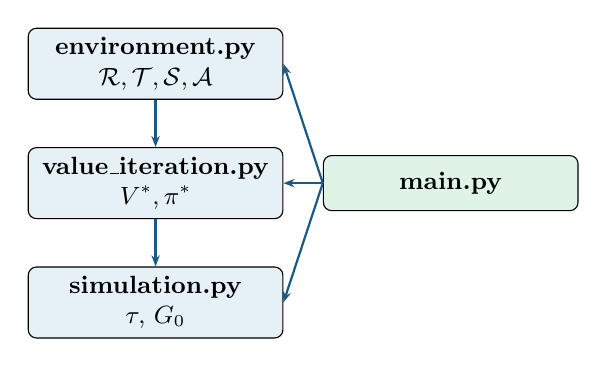
\begin{tikzpicture}[
        box/.style={draw,rounded corners=3pt,
                    fill=mathBlue!12,
                    text width=3.0cm, align=center,
                    font=\small, minimum height=0.7cm},
        arr/.style={-{Stealth[length=4pt]},
                    thick, mathBlue!70!black},
        node distance=0.6cm]
        \node[box] (env) {\textbf{environment.py}\\
          $\mathcal{R},\mathcal{T},\St,\Act$};
        \node[box, below=of env] (vi)
          {\textbf{value\_iteration.py}\\
           $\Vopt,\piopt$};
        \node[box, below=of vi] (sim)
          {\textbf{simulation.py}\\
           $\tau,\,G_0$};
        \node[box, right=0.5cm of vi,
              fill=goalGreen!15] (main)
          {\textbf{main.py}};
        \draw[arr] (env) -- (vi);
        \draw[arr] (vi)  -- (sim);
        \draw[arr] (main.west) -- (env.east);
        \draw[arr] (main.west) -- (vi.east);
        \draw[arr] (main.west) -- (sim.east);
      \end{tikzpicture}
      \end{center}
    \end{block}
    \begin{alertblock}{No extra dependencies}
      \texttt{pip install numpy} is sufficient.
    \end{alertblock}
  \end{columns}
\end{frame}

% ============================================================
\section{Summary}
% ============================================================

\begin{frame}{Summary -- Mathematical Role of Each File}
  \renewcommand{\arraystretch}{1.4}
  \begin{tabular}{>{\bfseries}p{3.0cm}
                  p{3.2cm}
                  p{5.8cm}}
    \toprule
    File & Math object & Key formula \\
    \midrule
    environment.py
      & $\St,\Act,\mathcal{R},\mathcal{T}$
      & $s=12r+c$;\;
        $\mathcal{R}(s,a)\in\{-100,-1,0\}$;\;
        $\sum_{s'}\mathcal{T}(s,a,s')=1$ \\[4pt]
    value\_iteration.py
      & $\Vopt,\piopt,Q^*$
      & $V_{k+1}(s)=\max_a[\mathcal{R}(s,a)
        +\gamma\,\mathcal{T}[s]\mathbf{V}_k]$;\;
        $\piopt(s)=\arg\max_a Q^*$ \\[4pt]
    simulation.py
      & $\tau,\,G_0$
      & $S_{t+1}=\arg\max_{s'}\mathcal{T}(S_t,A_t,s')$;\;
        $G_0=\sum_t R_{t+1}$ \\[4pt]
    main.py
      & Orchestration
      & Imports and calls all three modules \\
    \bottomrule
  \end{tabular}

  \bigskip
  \begin{columns}[T]
    \column{0.48\textwidth}
    \begin{block}{Key parameters}
      \begin{itemize}
        \item $|\St|=48$, $|\Act|=4$,
              $\gamma=0.99$, $\theta=10^{-8}$
        \item Optimal return: $G_0^*=-13$
        \item Optimal path: 13 steps
      \end{itemize}
    \end{block}
    \column{0.48\textwidth}
    \begin{block}{Theorems applied}
      \begin{itemize}
        \item Bellman optimality principle
        \item Banach contraction mapping
        \item Policy improvement theorem
      \end{itemize}
    \end{block}
  \end{columns}
\end{frame}

% Final frame
\begin{frame}[plain]
  \begin{center}
    \vspace{1.2cm}
    {\LARGE\bfseries Thank you!}\\[0.8em]
    {\large Cliff Walking MDP -- complete.}\\[1.2em]
    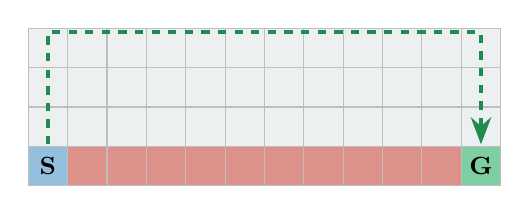
\begin{tikzpicture}[scale=0.50]
      \foreach \r in {0,1,2,3}{
        \foreach \c in {0,1,...,11}{
          \pgfmathparse{(\r==3)&&(\c>=1)&&(\c<=10)?1:0}
          \ifnum\pgfmathresult=1
            \fill[cliffRed!55]  (\c,3-\r) rectangle (\c+1,4-\r);
          \else
            \pgfmathparse{(\r==3)&&(\c==0)?1:0}
            \ifnum\pgfmathresult=1
              \fill[startBlue!50] (\c,3-\r) rectangle (\c+1,4-\r);
            \else
              \pgfmathparse{(\r==3)&&(\c==11)?1:0}
              \ifnum\pgfmathresult=1
                \fill[goalGreen!60] (\c,3-\r) rectangle (\c+1,4-\r);
              \else
                \fill[safeGray] (\c,3-\r) rectangle (\c+1,4-\r);
              \fi
            \fi
          \fi
          \draw[gray!50,thin] (\c,3-\r) rectangle (\c+1,4-\r);
        }
      }
      \node[font=\small\bfseries] at (0.5,0.5) {S};
      \node[font=\small\bfseries] at (11.5,0.5) {G};
      \draw[-{Stealth},thick,goalGreen!80!black,dashed,line width=1.5pt]
        (0.5,1.05)--(0.5,3.9)--(11.5,3.9)--(11.5,1.05);
    \end{tikzpicture}\\[0.6em]
    {\small Optimal path: Up $\to$ Right$\times11$ $\to$ Down
    \qquad $G_0^*=-13$}
  \end{center}
\end{frame}

\end{document}
